\documentclass{standalone}
%-----------------------------------------------------------------------------%
%%% Color %%%
\usepackage{xcolor}
\definecolor{myred}{RGB}{229,0,0}
\definecolor{myblue}{RGB}{0,98,144}
\definecolor{myyellow}{RGB}{246,182,50}
\newcommand{\red}[1]{\textcolor{myred}{#1}}
\newcommand{\blue}[1]{\textcolor{myblue}{#1}}
\newcommand{\yellow}[1]{\textcolor{myyellow}{#1}}
%-----------------------------------------------------------------------------%
%%% TikZ %%%
\usepackage{tikz}
% \usetikzlibrary{calc}
% \usetikzlibrary{positioning}
% \usetikzlibrary{patterns}
% \usetikzlibrary{fit}
% \usetikzlibrary{angles,quotes}
% \usetikzlibrary{intersections}
% \usetikzlibrary{decorations.markings}
%-----------------------------------------------------------------------------%

\begin{document}

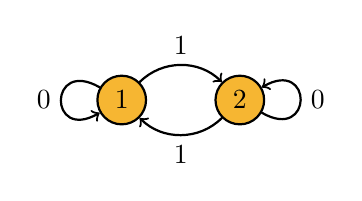
\begin{tikzpicture}[thick,line cap=round]
	\tikzstyle{bai}=[solid,circle,draw,inner sep=.8pt,fill=white];
	\tikzstyle{hei}=[solid,circle,draw,inner sep=.8pt,fill];
	\node[draw,circle,fill=myyellow] (1) at (0,0)   {$1$};
	\node[draw,circle,fill=myyellow] (2) at (1.5,0) {$2$};
	\draw[->] (1) to[out=045,in=135] node[above]{$1$} (2);
	\draw[->] (2) to[out=225,in=-45] node[below]{$1$} (1);
	\draw[->] (1) to[out=150,in=210,looseness=6] node[left]{$0$} (1);
	\draw[<-] (2) to[out=30,in=-30,looseness=6] node[right]{$0$} (2);
\end{tikzpicture}

\end{document}
